%
% Einstein Emulator User�s Manual (UP2)
%
% Code source LaTeX2e.
%
% Requiert un certain nombre de paquets (fournis avec la distribution de 
% i-Packages et sans doute la plupart des distributions):
% - palatino
% - hyperref
%
\documentclass[a4paper, english, 11pt]{article}
\usepackage{graphicx}
\usepackage{amssymb}
\usepackage{palatino}
\usepackage[applemac]{inputenc}
\usepackage[english]{babel}
\usepackage[T1]{fontenc}
\usepackage[top=2cm,bottom=2cm,left=1.5cm,right=1.5cm]{geometry}
\usepackage[
	bookmarksopen=true,
	pdfstartview=,
	pdftitle=Einstein\ Emulator\ User�s\ Manual,
	pdfauthor=Paul\ Guyot,
	pdfborder=false]{hyperref}
\title{\Huge Einstein Emulator\\
User�s Manual\\
�\\
\small{For Einstein Emulator UP2}}
\begin{document}
% Param�tres pour le document:
% ajustage de l'espace entre les caract�res pour la justification
\setlength{\emergencystretch}{12em}
% macro pour ins�rer une URL
\def\url#1{\href{#1}{\underline {\tt {#1}}}}
\maketitle
%
\newpage
\tableofcontents
\newpage
% espace entre les paragraphes
\parskip = 0.2in
\parindent = 0.0in
\pagestyle{myheadings}
\markright{Einstein Emulator User�s Manual}
\section{Introduction}
Einstein Emulator is a Newton N2 platform (MP2x00, eMate 300) emulator.

The particularity of this platform is that the core of the system is not the central processor unit (CPU) but the ASIC, called Voyager (this is why the N2 platform is also called the Voyager platform, opposed to earlier Newtons based on the Runt ASIC).

The Voyager chip was used as a limit between dreams and reality when it came to the future of the Newton platform after it was abandonned by Apple Computer, Inc. This chip was produced by Cirrus and apparently designed by Apple and Cirrus, as long with other chips in the Newton such as the PCMCIA controllers. No publicly available documentation about these chips exist and it is unlikely that Cirrus will produce any additional chip. Consequently, until recently, the Newton platform was limited to the limited existing set of working units.

Einstein Emulator was designed with little knowledge of the ASIC, even if some  important bits are emulated. The emulator takes advantage of the way the Newton operating system handles hardware drivers and, without modifying the ROM, it replaces the original drivers with drivers hooked into the emulator, thus bypassing most accesses to the ASIC.

This technique was presented during the first Worldwide Newton Conference:
\url{http://wwnc.newtontalk.net/program/paulguyot/}

\newpage
\section{Requirements}

To run Einstein Emulator, you will need:
\begin{itemize}
\item a computer running MacOS X
\item a NewtonOS 2.1 ROM
\end{itemize}

The binary for MacOS X was compiled with gcc and optimized for G4. I highly suggest to quit as many programs as possible and to quit Classic (which typically sucks 30\% of the CPU after you used Newton-development programs). It works reasonnably well on my PowerBook, a PowerBook G4 1.67 GHz.

\begin{itemize}
\item Einstein Emulator requires an MP2x00 US, an MP2x00 D or an eMate 300 ROM image.
\end{itemize}

Instructions about how to extract the ROM are available in the next section.

PLEASE DO NOT ASK ME FOR A ROM FILE. I will not provide you with any.
NewtonOS ROM is copyright by Apple Computer, Inc and licensors.

\newpage
\section{Extraction of the ROM from your Newton}

Two methods are available: via a serial line or via TCP/IP (i.e. via an Ethernet access).

\subsection{Hammer/Newtsbug (serial line)}

Using a low-level debugger such as Hammer or Newtsbug, you can make a dump of the memory. This is slow and works over the serial line.

\underline{Requirements:}
\begin{itemize}
\item A computer running in Classic or MacOS < X
\item Hammer or Newtsbug (they can be found on UNNA, \url{http://www.unna.org/})
\item A serial connection between your Newton and the Mac:
\begin{itemize}
\item a built-in serial port for computers booting in MacOS < X
\item or a USB to Serial port adapter compatible with Classic.
\end{itemize}
\end{itemize}

\underline{Steps:}
\begin{itemize}
\item Install Debugger Connection or Newtsbug Connection package on your Newton.
\item Plug the Newton with the Mac using the serial line.
\item Run Hammer or Newtsbug on the Mac.
\end{itemize}
A standard get file dialog appears: choose the debugging image corresponding to your Newton (Senior CirrusNoDebug image, Senior DCirrusNoDebug image or Newt KNoDebug image for the MP2x00 US, MP2100 or eMate 300 respectively).
\begin{itemize}
\item Tap the Debugger Connection or Newtsbug Connection package on your Newton and choose connect.
\item On the Mac, once the connection is established, choose Save Memory from the File menu.
\item Save memory between 0 and 00800000 (8 MB).
\end{itemize}

Wait.

\subsection{ROM Dumper (TCP/IP)}

ROM Dumper is a faster approach but requires an internet connection between your Mac (or any Unix computer) and your Newton.

\underline{Requirements}
\begin{itemize}
\item A working TCP/IP or Internet connection between your Newton and your Mac.
\end{itemize}

\underline{Steps:}
\begin{itemize}
\item Install provided ROM Dumper package on your Newton.
\item Tap the ROM Dumper icon in the Extras Drawer.
\item Tap start.
\item If your Newton isn�t connected to the Internet yet, choose a connection method. It�s also the time to insert your Ethernet/WiFi card.
\item Note the IP of the Newton (ROM Dumper mentions it).

\begin{center}
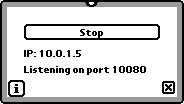
\includegraphics[width=12cm]{ROMDumper.png}\\
\emph{ROM Dumper listening}
\end{center}

\item Launch Einstein Emulator (the GUI version).
\item Choose Dump ROM from the Einstein menu.

\begin{center}
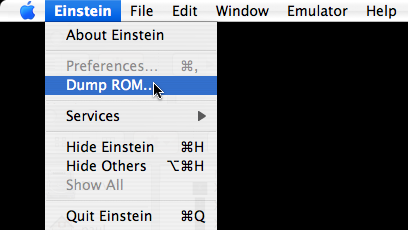
\includegraphics[width=12cm]{DumpROMMenuItem.png}\\
\emph{Dump ROM Menu Item}
\end{center}

\item Type the IP address of your Newton.

\begin{center}
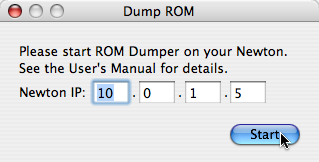
\includegraphics[width=12cm]{DumpROMPanel.png}\\
\emph{Dump ROM Panel}
\end{center}

\item Click start.
\item Mention where to save the Newton ROM. Be careful not to erase previously dumped ROM file if you are dumping the ROM of several different Newton models.
\item Wait (a little bit).
\end{itemize}

The emulator will be configured to use the newly dumped ROM.

Alternatively, you can use nc(1) command line tool.

\newpage
\section{Using the CLI flavor}

The CLI flavor should mainly be used to access the log and/or the monitor mode. It is therefore intended for developers. Users could simply double-click the MacOS X application.

\begin{itemize}
\item Name the ROM dump either:
717006 (MP2x00 US)
737041 (MP2100 D)
747129 (eMate 300)

\item Put the file in the data directory, next to Einstein.rex file (Einstein.rex is
the ROM Extension for Einstein emulator, it includes Einstein drivers and
Frank Gruendel's NewtTest program).

\item Then, in the Einstein directory, launch Einstein with:
\verb|$ ./einstein --machine=XXXX data|
\end{itemize}

where XXXX should be either:
717006 (for a MP2x00 US)
737041 (for a MP2100 D)
747129 (for an eMate 300)

\subsection{Options}
\verb|./einstein --help| will print some help about the options. The options are summarized below:

\verb|--audio| or |-a|\\
Select the audio driver (null, portaudio or coreaudio). \verb|--audio=null| will disable sound. \verb|--audio=portaudio| will choose portaudio sound driver. Default is coreaudio.


\verb|--screen| or \verb|-s|\\
This option is useless now as the only available screen driver is x11. Framebuffer support may be added later.

\verb|--width|\\
Set the width of the screen (in portrait mode). Default is 320.

\verb|--height|\\
Set the height of the screen (in portrait mode). Default is 480.

\verb|--log| or \verb|-l|\\
Set the log file. Default is to not log. This option is incompatible with --monitor.

\verb|--restore| or \verb|-r|\\
This option is unimplemented.

\verb|--machine| or \verb|-m|\\
Set the machine. Choose 717006 for a MP2x00 US, 737041 for a MP2100D or 747129 for an eMate 300. \verb|--machine| option can be omitted with a 717006 ROM file.

\verb|--monitor|\\
Run in monitor mode.

\verb|--ram|\\
Set the RAM size in 64 KB increment. 1 will mean 64 KB of RAM. 64 is the default setting (4 MB). The maximum is 255 (nearly 16 MB).

\subsection{Commands}

Using the cli flavor, you will be provided with a prompt. Typing help will provide a small help about the available commands.

\subsection{Logging}

Quite a large amount of log lines are generated by the emulator. These are used during the development of Einstein emulator. It also helps to understand what�s going on.

Starting with UP2 release, you can generate log lines from NewtonScript calling the |Einstein:Log|�global function.

E.g.:
\begin{verbatim}
|Einstein:Log|(�Hello World�)
\end{verbatim}

will display \texttt{Hello World} in the log.

Please note that your string is converted to ISO-8859-1 before being printed, so non latin characters will not be printed properly in the log.

\subsection{Monitor mode}

The monitor mode uses a disassembler from the NetBSD project (the kernel disassembler for the arm32 port). You start in monitor mode by specifying the --monitor option to the command line program.

The monitor mode can be considered as an enhanced low-level debugger. The help command displays a short help for the available commands.

One of the main advantage of the monitor is that you can set breakpoints. You can also halt the emulator by calling the |Einstein:BreakInMonitor| global function (it doesn�t take any parameter).

The following breakpoints are enabled by default:
\begin{itemize}
\item NewtonOS UND instructions to pass strings to the debugger (typically followed by a reboot). They are executed (i.e. the Newton will reboot), but the Newton is halted and the string is printed to the monitor.
\item Some violations that shouldn't happen.
\end{itemize}

You cannot use \verb|--log| option with \verb|--monitor| because in monitor mode, the log is always enabled. You can save the log to a file (it scrolls on the monitor screen).

The monitor mode uses a file with symbols. This file should be named after the ROM file, e.g. 717006.symbols. The syntax is:

\verb|address <tab> symbol <tab> comment|

Addresses should be sorted.

This file is very easy to generate from the debugger images that are used with
Hammer and Newtsbug. Use Newton C++ Tools DumpAIF program with the -s option to dump the list of symbols. Then you can process all the lines with research and replace or sed or awk at your convenience. The symbols can be unmangled with Unmangle tool coming with MPW.

\newpage
\section{Notes on flash}

Starting with DR1, Einstein Emulator saves the flash to a file.

This file is either in the "Einstein Emulator" directory of the "Application Support" of the Library directory in your home directory (Cocoa flavor) or in the data directory passed as the option of the CLI flavor.

The ROM checksum is computed at startup and the flash block 0 is filled with proper checksum values to prevent the operating system from deciding to erase the flash.

If you swap the ROM boards on a hardware unit, NewtonOS will erase the flash.

With this checksum calculation, even if you choose another ROM file, the OS will not erase the internal store. This may introduce problems:
- system patches only work with the ROM they were designed for
- sorting is different on German and US units.

Consequently, it is highly suggested to remove the flash file between virtual ROM swaps.

Also, please note that if you set a breakpoint before the system did compute the checksum, it might think that the ROM board changed and decide to erase the internal store.

The flash is synchronized to disk when it is powered off (either when the unit is powered off or when just the flash chips are powered off by the OS). Depending on the host operating system, it may be flushed to disk between power offs.

Einstein Emulator emulates 8 MB of flash. This is the maximum that can be emulated on two banks of 4 MB each. There seems to be another possible bank for flash. However, one cannot choose the flash size yet.

\newpage
\section{Notes on RAM}


Starting with DR2, the emulator comes with a new option to specify the size of the RAM in 64 KB units. 64 64 KB units is what is used by default (4 MB, what can be found in MP2100s).

The highest amount of RAM that can be used there seems to be 255 units of 64 KB (nearly 16 MB). There seems to be another RAM bank but it isn't supported yet.

Please note that RAM and ROM are backed with RAM on the host system.
Additionally, because of threaded emulation, all the ROM and the RAM is backed with a zone 4 times bigger to include decoded instruction data and function pointers.

In other words, emulating a regular MP2100 with the 16 MB of ROM of the emulator requires approximatively 100 MB on MacOS X.

\newpage
\section{Notes on package installation}

Package installation is slow, because of the way the emulator communicates with the Newton. Basically, the package is sliced in packets of 236 bytes and these packets are sent to the NewtonScript task via events. A progress window has been added with DR2, but it only represents the downloading part of the process. The window is closed when the package is being sucked from the binary. This can take quite a lot of time. Additionally, it may fail if the free space on the default store is less than twice the size of the package.

A more efficient way would be to perform a SuckPackageFromEndpoint and to emulate an endpoint instead. It might be more interesting to write AppleTalk bindings and use the regular package installer programs available.

Package installation can be cancelled by pressing the stop button. However, this does not stop the download of the package.

\newpage
\section{Notes on keyboard emulation}

Keyboard is emulated with both Cocoa and X11 screen managers. eMate top row keys are ESC (close button) and F1 to F12.

With the Cocoa interface, keys are captured whenever the mouse is over the Newton emulator's screen.

Unsurprisingly, the Newton supports a keypad (keypad keys are not the same
as their equivalent on the main keyboard). The Newton also gets other function keys and some software could take advantage of it (my own keyboard only has 12 functions keys, so I wasn't able to test it).

However, there are several limitations:
\begin{itemize}
\item auto-key events aren't sent at all with X11 interface. Instead, Einstein Emulator benefits from X11 built-in auto-repeat events and the Newton gets events as if the keys were pressed and released repeatedly (as regular X11 programs do).
\item auto-key events don't work with modifier keys. As a result (I think), the shortcut help isn't shown if you maintain the command key.
\item right shift (and possibly right control and right option) keys aren't captured by the Cocoa interface (they aren't captured by the X11 interface, but I don't think X11 sends the information anyway). I believe this is a limitation of MacOS X (for the record, Cocoa APIs don't export this information, but Carbon APIs do, and it's what I use).
\item caps lock isn't emulated exactly the way it should be. With the Cocoa interface, the Newton sees presses and releases whenever the caps lock state changes.
\item shortcuts defined by X11.app aren't captured. Others are passed to the Newton. This doesn't happen with the Cocoa interface (you can send command-Q to the Newton for example).
\item X11 keycodes are translated for Apple X11 (basically, I substract 8 from the X11 keycode to obtain the Mac/Newton virtual key code). Future release might support other keycodes translations for other X11 servers.
\item F11 and F12 keys (backlight and power) buttons don't work with the eMate's ROM.
\item so far, pressing a key will wake the Newton up.
\item The keyboard emulation uses the same channel as the package installation. Consequently, typing is difficult if not impossible when you are installing a package.
\end{itemize}

\newpage
\section{Notes on the Cocoa interface}

The first time you launch the Cocoa application, you will be welcomed by the Setup Window. This window lets you configure the emulator. Choose the ROM image you have previously downloaded from your Newton by clicking the appropriate �Choose...� button.

\begin{center}
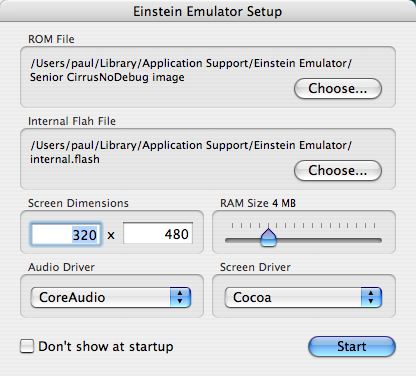
\includegraphics[width=12cm]{SetupWindow.png}\\
\emph{Setup Window}
\end{center}

Packages can be installed by dropping them on the screen.

The interface includes some artwork by Michael Vac�k.

\newpage
\section{Additional developer notes}

Since DR1, the Einstein Rex defines a gestalt entry to distinguish hardware units from Einstein.

The following C declaration could be used to determine, with Gestalt, if your native code is running under Einstein Emulator. This selector is not defined in hardware units.

\begin{verbatim}
#define kGestalt_Einstein_Base            0x03000001
#define kGestalt_Einstein_EmulatorInfo    (kGestalt_Einstein_Base + 1)

// Version
#define	kDR1Version	0x00010000
#define	kDR2Version	0x00010001
#define	kUP1Version	0x00010002
#define	kUP2Version	0x00010003

// Host CPU.

struct SGestaltEinsteinEmulatorInfo
{
    KUInt32     fVersion;                   ///< Current version.
};
\end{verbatim}

The fVersion field is in MacOS/NewtonOS version format (like ROMVersion in the system info). High 16 bits design the major version and low 16 bits the minor version (UP1 hence is represented as 1.2).

Alternatively, you can determine this information with the following NewtonScript code:

\begin{verbatim}
constant kGestaltArg_EinsteinEmulatorInfo := '[0x03000002, [struct,long], 1];
constant kDR1Version := 0x00010000;
constant kDR2Version := 0x00010001;
constant kUP1Version := 0x00010002;
constant kUP2Version := 0x00010003;

/**
 * Determine if we're under Einstein Emulator, and if so, its version.
 *
 * @return	nil if we're on a hardware unit, the Einstein Emulator version
 *			otherwise.
 */
DefConst('kDetermineEinsteinEmulatorVersionFn,
    func()
    begin
        local theResult := Gestalt(kGestaltArg_EinsteinEmulatorInfo);
        if (theResult) then return theResult[0] else return nil;
    end);
\end{verbatim}

Additionally, the REx defines a global function to get a string representation of the version of Einstein. It's GetEinsteinVersionString().

\newpage
\section{Known problems}

\begin{itemize}
\item Serial ports are not emulated.
\item PCMCIA cards are not emulated. The sockets aren�t entirely emulated yet.
\item Some slow-downs may be experienced after a while. I believe it's related to interruptions.
\item The sound volume is reported to be settable by software but the emulator ignores changes in the volume (except when the sound is off on the Newton).
\item Sound input isn't emulated.
\item Installing a package by dropping it on the Cocoa screen with a path containing a non US ASCII characters fails.
\item An error occurs when trying to install system patches.
\end{itemize}

Please drop me a line (\url{mailto:pguyot@kallisys.net}) if you experience a problem which is not in this list.

\newpage
\section{Changes History}

5/06/05 UP2
\begin{itemize}
\item Rewrote the PortAudio interface.
\item Added a CoreAudio sound manager. This is now the default sound manager.
\item Fixed a problem in Tiger: the screen wasn�t updated when the mouse button was down.
\item Transform the README document into this User�s Manual.
\item Added NewtonScript global functions to log lines or to break into the monitor.
\item User data is now imported from the AddressBook if available, or via the account (Unix method is also implemented and has been tested).
\item The time zone is now set to match the host time zone. This is achieved by setting the location on the Newton (instead of default which is San Francisco on US units). The location is chosen as being either the city of the owner (if found in the AddressBook and if the time zone matches), a city in the same region or state, a city of the country of the owner or whatever city is in the same time zone. A random location is created in the unlikely case the host time zone doesn�t exist on the Newton.
\item Created a GUI to dump the ROM via TCP/IP instead of using nc(1) in the Terminal.
\item Emulation of 2 PCMCIA sockets. I discovered that NewtonOS will corrupt memory if I try to emulate more than 2. Interruption aren't emulated yet.
\item Emulation of the serial number ROM Chip. The NewtonID is set to 0000-4E65-7774-6F6E for now.
\item Fixed a bug yielding to a total loss of changes between reboots. Flash files saved in UP1 are actually empty and will be "factory-recalibrated".
\item The preferences are now saved to file and the setup window can be skipped.
\item Alerts that were previously logged in the Console are now reported with a NSAlert.
\item Added primitive NIE bindings (incomplete).
\item X11 interface now works with Familiar Linux� X11 server.
\item Recompiled with gcc-4.0.
\end{itemize}

5/3/2005	UP1
\begin{itemize}
\item Added a Cocoa screen manager and a whole Cocoa application around it.
\item Added keyboard support.
\item Improved the way events are transmitted from the host to the Newton.
\item X11 screen manager can now cope with most (any?) visual (using XAllocColor). Please note that 8 bits TrueColor cannot represent either the 16 shades of gray or the 16 shades of green.
\end{itemize}

22/2/2005	ZP1
\begin{itemize}
\item Fixed a bug in the cli application code.
\item Fixed a bug in the way breakpoints are parsed.
\item Improved the package installation by reporting progress on the installation itself (in addition to progress of the transfer).
\item Allowed several packages to be installed in a row.
\item Added a watch command to watch parameters and log the result.
\item Improved screen interface by making it endianness-agnostic.
\item Improved flash by making it endianness-agnostic.
\item Fixed bugs in the X11 interface, including better multi-threaded code.
\item X11 display now is endianness-agnostic and works with both 24 and 15 bits depth (millions and thousands of colors).
\item Flash now uses mmap(2) and associated calls.
\item RTC delta is now initialized so that the Newton is set to host time at boot.
\item Fixed a bug that prevented the Newton to be powered off more than once.
\item Memory and ROM are now swapped on little-endian machines, thus avoiding unnecessary conversions during each access.
\item Many optimizations.
\end{itemize}

4/2/2005	DR2
\begin{itemize}
\item Flash erase method now takes the block size into account. This actually was what prevented system patches to be installed.
\item Fixed a bug in the emulator to Newton events transmission. This actually prevented packages bigger than 16 KB from being installed.
\item Fixed an optimization in the way interruptions were masked.
\item Improved the package installation by adding a progress indicator. Additionally, installation can now be cancelled by pressing the stop button.
\item Fixed a bug related to VBOs in package installation (the VBO cache wasn't cleaned).
\item Improved segmented event transmission by preventing the Newton to power off.
\item New flash is now initialized with both ROM checksum and factory calibration data. To take advantage of this feature, you must delete the flash file created by previous releases of Einstein Emulator.
\item Added an option to choose RAM size (between 64K and 16320K).
\item Fixed a problem related to the way quit command worked.
\end{itemize}

28/1/2005	DR1
\begin{itemize}
\item New monitor mode (option: --monitor) to directly control the emulator and debug programs.
\item The interface was reworked to support the new monitor mode.
\item Support for arbitrary screen sizes. Please note that: (a) you'd better not use a screen smaller than the original (320x480) and (b) the size should be provided in portrait mode (i.e. width should be smaller than height) and (c) you need to click on the lower-right corner for pen alignment (this typically doesn't do anything, maybe I should disable it), so you'd better provide a size that is not too big for your screen. Size is provided with new --width and --height options.
\item Added a command to execute arbitrary NewtonScript command line (ns <command>)
\item Added a command to install a package (install <path>)
\item Flash is now saved when the power goes off.
\item Fixed the power switch button (it no longer generates an event when the Newton is off).
\item Added support for NewtonOS debug undefined instructions.
\item Added computation of the ROM checksums. The checksums are written to flash on startup so NewtonOS will not erase the flash accross updates of the emulator (and specifically of the REX).
\item Updated NewtTest to 1.1g.
\end{itemize}

16/1/2005	DP3
\begin{itemize}
\item Optimized the code (the emulator is now 30\% faster).
\item Wrote a TCP/IP utility to dump the ROM.
\item Fixed a bug in many instructions leading to a weird way to display floating point numbers (and probably other elements).
\item Made the REx and the Emulator work with other 2.1 Newtons.
\item Began support for checksumming of the ROM.
\item Began support for GPIO including support for the power switch (doesn't work very well yet) and support for the backlight.
\item Removed the custom version string from the Rex (it was only displayed on the emate).
\item Rewrote the CLI application, disabling log by default.
\end{itemize}

3/1/2005	DP2
\begin{itemize}
\item Fixed the rotation problem
\item Included Frank Gruendel's NewtTest program
\item Wrote a README file.
\end{itemize}

2/1/2005	DP1 Initial release

\newpage
\section{License}

Einstein Emulator is copyright 2005 by Paul Guyot.
Cocoa interface artworks are copyright 2003-2005 by Michael Vac�k.
It is provided as is, without any warranty of any kind.

Einstein Emulator includes portaudio v19 (from CVS).

\begin{verbatim}
/*
 * PortAudio Portable Real-Time Audio Library
 * Latest Version at: http://www.portaudio.com/
 *
 * Copyright (c) 1999-2000 Phil Burk and Ross Bencina
 *
 * Permission is hereby granted, free of charge, to any person obtaining
 * a copy of this software and associated documentation files
 * (the "Software"), to deal in the Software without restriction,
 * including without limitation the rights to use, copy, modify, merge,
 * publish, distribute, sublicense, and/or sell copies of the Software,
 * and to permit persons to whom the Software is furnished to do so,
 * subject to the following conditions:
 *
 * The above copyright notice and this permission notice shall be
 * included in all copies or substantial portions of the Software.
 *
 * Any person wishing to distribute modifications to the Software is
 * requested to send the modifications to the original developer so that
 * they can be incorporated into the canonical version.
 *
 * THE SOFTWARE IS PROVIDED "AS IS", WITHOUT WARRANTY OF ANY KIND,
 * EXPRESS OR IMPLIED, INCLUDING BUT NOT LIMITED TO THE WARRANTIES OF
 * MERCHANTABILITY, FITNESS FOR A PARTICULAR PURPOSE AND NONINFRINGEMENT.
 * IN NO EVENT SHALL THE AUTHORS OR COPYRIGHT HOLDERS BE LIABLE FOR
 * ANY CLAIM, DAMAGES OR OTHER LIABILITY, WHETHER IN AN ACTION OF
 * CONTRACT, TORT OR OTHERWISE, ARISING FROM, OUT OF OR IN CONNECTION
 * WITH THE SOFTWARE OR THE USE OR OTHER DEALINGS IN THE SOFTWARE.
 *
 */
\end{verbatim}

Einstein Emulator also includes NetBSD arm disassembler.

\begin{verbatim}
// $NetBSD: disassem.c,v 1.14 2003/03/27 16:58:36 mycroft Exp $
//
// Copyright (c) 1996 Mark Brinicombe.
// Copyright (c) 1996 Brini.
//
// All rights reserved.
//
// Redistribution and use in source and binary forms, with or without
// modification, are permitted provided that the following conditions
// are met:
// 1. Redistributions of source code must retain the above copyright
//    notice, this list of conditions and the following disclaimer.
// 2. Redistributions in binary form must reproduce the above copyright
//    notice, this list of conditions and the following disclaimer in the
//    documentation and/or other materials provided with the distribution.
// 3. All advertising materials mentioning features or use of this software
//    must display the following acknowledgement:
//	This product includes software developed by Brini.
// 4. The name of the company nor the name of the author may be used to
//    endorse or promote products derived from this software without specific
//    prior written permission.
//
// THIS SOFTWARE IS PROVIDED BY BRINI ``AS IS'' AND ANY EXPRESS OR IMPLIED
// WARRANTIES, INCLUDING, BUT NOT LIMITED TO, THE IMPLIED WARRANTIES OF
// MERCHANTABILITY AND FITNESS FOR A PARTICULAR PURPOSE ARE DISCLAIMED.
// IN NO EVENT SHALL BRINI OR CONTRIBUTORS BE LIABLE FOR ANY DIRECT,
// INDIRECT, INCIDENTAL, SPECIAL, EXEMPLARY, OR CONSEQUENTIAL DAMAGES
// (INCLUDING, BUT NOT LIMITED TO, PROCUREMENT OF SUBSTITUTE GOODS OR
// SERVICES; LOSS OF USE, DATA, OR PROFITS; OR BUSINESS INTERRUPTION)
// HOWEVER CAUSED AND ON ANY THEORY OF LIABILITY, WHETHER IN CONTRACT, 
// STRICT LIABILITY, OR TORT (INCLUDING NEGLIGENCE OR OTHERWISE) ARISING IN
// ANY WAY OUT OF THE USE OF THIS SOFTWARE, EVEN IF ADVISED OF THE
// POSSIBILITY OF SUCH DAMAGE.
\end{verbatim}

\end{document}
